% Provenance (never printed): see sources/outline_sources.md (Year 2: the Himalaya and Tibet;
% the Andes; crustal thickening and plateaus). Himalayan units, thrusts and rates after Lave
% and Avouac (2000), Ader et al. (2012), Cattin et al. (2001), Dong et al. (2026, STDS);
% Asian extrusion after Jiao et al. (2023); Tibetan rifts after Wang et al. (2021); Central
% Andes after Gerbault et al. (2005); flat slabs after Gauthier et al. (2024). Relief from
% ETOPO1 (figdata/bachelor-2/plateaus.py); plate velocities from NNR-MORVEL56 (Book 2 ledger
% row nnr56:poles). Exercise and problem values in the Book 4 scratch calculator
% calc/ch14.py.
\chapter{مقارنة بين حزام تصادمي وحزام أنديزي}\label{ch:b2:himalaya-andes}

على الأرض هضبتان ترتفعان أكثر من أربعة كيلومترات على مدى مئات الكيلومترات.
فقد ارتفعت التبت حيث اصطدمت الهند بآسيا، قارتان التقتا بعد أن زال المحيط الذي
كان بينهما. وارتفعت الألتيبلانو حيث لا تزال صفيحة محيطية، صفيحة نازكا، تنزلق
تحت أمريكا الجنوبية، دون أن تصل أي قارة على الإطلاق. محرّكان مختلفان بنيا
تضاريسين متشابهتين. يفكّك هذا الفصل الحزامين، ويقيس مقدار ما بلغته قشرتهما من سمك
ولماذا، ويسأل عمّا يمنعهما من الارتفاع أكثر.
% ledger: lave00:setting, gerbault05:andes, data:b4-etopo-tibet, data:b4-etopo-andes

\begin{recall}
\textbf{من مجلد المرحلة الثانوية}: التصادم القاري والدرز؛ وانجراف الهند
نحو الشمال، وتباطؤه، والعمر المختلف فيه للتصادم؛ وهضبة التبت التي يبلغ ارتفاعها نحو
\qty{4600}{m} فوق قشرة سمكها نحو \qty{70}{km}. \textbf{من مجلد السنة الأولى}:
توازن إيري وصفيحة بوغيه؛ والهوامش النشطة، والكتلة المندسّة، والقوس البركاني
وفجوة القوس والخندق؛ وسرعات الصفائح من السرعات الزاوية؛ وقانون بايرلي؛ وقدر
العزم. \textbf{من \cref{ch:b2:crustal-melting}}: الليوكوغرانيتات الهيمالايية.
\textbf{من \cref{ch:b2:alpine-orogen}}: \omterm{def:b2:alpine-orogen:orogen}{الأوروجين}، \omterm{def:b2:alpine-orogen:nappes}{والغطاء الزاحف}، \omterm{def:b2:alpine-orogen:decollement}{وسطح الانفصال}، والتكتونية الرقيقة
\omterm{def:b2:alpine-orogen:skin}{والسميكة الجلد}، \omterm{def:b2:alpine-orogen:ftb}{وحزام الطيّات والدفع}، \omterm{def:b2:alpine-orogen:foreland}{والحوض الأمامي الجبلي}، \omterm{def:b2:alpine-orogen:balanced}{والمقاطع العرضية المتوازنة}.
\end{recall}

\begin{definition}[الأوروجين التصادمي؛ الأوروجين من النمط الأنديزي]\label{def:b2:himalaya-andes:types}
\emph{الأوروجين التصادمي}\index{الأوروجين التصادمي} أوروجين بناه تقارب
هامشين قاريين بعد استهلاك المحيط الذي كان بينهما؛ ومحوره درز.
و\emph{الأوروجين من النمط الأنديزي}\index{الأوروجين من النمط الأنديزي} أوروجين مبني على الصفيحة
العليا لنطاق اندساس محيطي--قاري، بينما يستمر الاندساس تحته؛ ومحوره
قوس بركاني.
\end{definition}


\section{الهند في مواجهة آسيا}\label{sec:b2:himalaya-andes:himalaya}

التقت الهند بالحافة الجنوبية لأوراسيا قبل نحو 50 مليون سنة على امتداد درز إندوس--تسانغبو،
الذي يسمّى أيضًا درز إندوس--يارلونغ؛ ولا يزال التاريخ الدقيق موضع خلاف، كما بيّن
مجلد المرحلة الثانوية. ولم يتوقف التقارب. فاليوم تقترب الهند وآسيا إحداهما من الأخرى
بنحو \qty{40}{mm} في السنة؛ ومن السرعات الزاوية لنموذج الصفائح NNR-MORVEL56،
تتحرك الهند بسرعة \qty{45}{mm} في السنة بالنسبة إلى أوراسيا عند \ang{28} شمالًا و\ang{85} شرقًا، نحو
\ang{22} شرق الشمال. ولا يُستوعب في الهيمالايا إلا جزء من تلك الحركة. فعبر نيبال،
تُظهر محطات GPS أن الهند وجنوب التبت تتقاربان بمعدل $17.8 \pm \qty{0.5}{mm}$ في السنة في
الوسط والشرق و$20.5 \pm \qty{1}{mm}$ في السنة في الغرب: أي نحو نصف المجموع. والباقي
موزّع على التبت وبقية آسيا.
% ledger: lave00:setting, najman21:collision-age, jiao23:extrusion, nnr56:poles, ader12:rates, ader12:mht
% values (plateaus.py): v_india_eurasia 44.99 mm/yr, azimuth 21.65

تُظهر الخريطتان أدناه الحزامين بخطوط الكنتور نفسها، والشرائط التي يقطعهما هذا
الفصل على امتدادها.

\begin{omfigure}
\centering
% ledger: data:b4-etopo-tibet, data:b4-etopo-andes
\begin{tikzpicture}
\begin{axis}[name=tib, scale only axis, width=8.0cm, height=4.8cm, xmin=75, xmax=100,
  ymin=25, ymax=40, xlabel={خط الطول (\unit{\degree} شرقًا)}, ylabel={خط العرض (\unit{\degree} شمالًا)},
  tick label style={font=\scriptsize}, label style={font=\small}, xtick={75,80,...,100},
  ytick={25,30,...,40}, title={\small الهيمالايا والتبت}]
\addplot[omThm!35, line width=0.3pt] table[x=lon, y=lat] {figdata/out/bachelor-2-plateaus-tc2000.dat};
\addplot[omThm!90!black, line width=0.4pt] table[x=lon, y=lat] {figdata/out/bachelor-2-plateaus-tc4000.dat};
\draw[black, densely dashed, line width=0.9pt] (axis cs:86,25) rectangle (axis cs:90,40);
\node[font=\scriptsize, fill=white, fill opacity=0.85, text opacity=1, inner sep=1pt] at (axis cs:80,26.2) {سهل الغانج};
\node[font=\scriptsize, fill=white, fill opacity=0.85, text opacity=1, inner sep=1pt] at (axis cs:94.5,33.5) {هضبة التبت};
\node[font=\scriptsize, fill=white, fill opacity=0.85, text opacity=1, inner sep=1pt] at (axis cs:83,39.2) {تاريم};
\end{axis}
\begin{axis}[at={(tib.east)}, anchor=west, xshift=1.6cm, scale only axis, width=3.6cm,
  height=4.8cm, xmin=-75, xmax=-60, ymin=-30, ymax=-10,
  xlabel={خط الطول (\unit{\degree})}, tick label style={font=\scriptsize},
  label style={font=\small}, xtick={-75,-70,-65,-60}, ytick={-30,-25,...,-10},
  title={\small الأنديز الوسطى}]
\addplot[blue!60!black, line width=0.45pt] table[x=lon, y=lat] {figdata/out/bachelor-2-plateaus-ac0.dat};
\addplot[omThm!35, line width=0.3pt] table[x=lon, y=lat] {figdata/out/bachelor-2-plateaus-ac2000.dat};
\addplot[omThm!90!black, line width=0.4pt] table[x=lon, y=lat] {figdata/out/bachelor-2-plateaus-ac4000.dat};
\draw[black, densely dashed, line width=0.9pt] (axis cs:-75,-21) rectangle (axis cs:-60,-19);
\node[font=\scriptsize, fill=white, fill opacity=0.85, text opacity=1, inner sep=1pt] at (axis cs:-73,-25) {الهادئ};
\end{axis}
\end{tikzpicture}
\par\smallskip{\small تضاريس الحزامين من نموذج ETOPO1، تفصل بين عقد الشبكة \qty{0.1}{\degree}:
خطوط كنتور عند \qty{2000}{m} (فاتحة) و\qty{4000}{m} (داكنة)، وخط الساحل في الخريطة
اليمنى. خطوط العرض في الخريطة اليمنى سالبة جنوب خط الاستواء، وخطوط الطول سالبة غرب
غرينتش. والمستطيلان المتقطّعان هما شريطا المقطعين اللاحقين: \qtyrange{86}{90}{\degree} شرقًا
عبر الهيمالايا والتبت، و\qtyrange{19}{21}{\degree} جنوبًا عبر الأنديز الوسطى.}
\end{omfigure}

\subsection{الوحدات والصدوع الدفعية}

من سهل الغانج شمالًا، يعبر مقطع عبر الهيمالايا ركامًا من الصفائح الدفعية
المقتطعة من الهامش الشمالي للهند، تفصل بينها صدوع تمتدّ على طول السلسلة.
\begin{itemize}
\item \emph{المنخفض الأمامي الهندي--الغانجي} هو \omterm{def:b2:alpine-orogen:foreland}{الحوض الأمامي الجبلي} للهيمالايا؛ ويحتجز جزءًا من
الحطام المحتوت من السلسلة.
\item \emph{نطاق ما تحت الهيمالايا}، أي تلال سيواليك، مكوَّن من مولاس ذلك الحوض،
من الحجر الطيني إلى الكونغلوميرا، وعمرها من الميوسين المتأخر إلى البليستوسين، وسمكها من 3500 إلى \qty{5500}{m}،
ترسّبت بين 14 و\qty{1}{Ma}، ثم كُشطت عند جبهة السلسلة وطُويت فوق
سطح انفصال: حزام طيّات ودفع رقيق الجلد. وحافته الجنوبية هي \emph{الصدع الدفعي الجبهي
الرئيسي} (MFT).
\item \emph{الهيمالايا الصغرى}، وهي صخور متوسطة الدرجة التحوّلية، تقع بين
\emph{الصدع الدفعي الحدّي الرئيسي} (MBT) أسفلها و\emph{الصدع الدفعي المركزي الرئيسي} (MCT) أعلاها.
\item \emph{متتالية الهيمالايا الكبرى} (الهيمالايا العليا) فوق MCT مكوّنة من
صخور تحوّلية عالية الدرجة، منصهرة جزئيًا: ميغماتيتات
\cref{ch:b2:crustal-melting} وليوكوغرانيتاته، التي انصهرت بعد التصادم بنحو 30 مليون سنة.
\item \emph{متتالية الهيمالايا التيثيسية}، وهي رواسب غير متحوّلة أو ضعيفة التحوّل من
الهامش السلبي القديم للهند، ترتكز على متتالية الهيمالايا الكبرى على امتداد
\emph{منظومة انفصال جنوب التبت} (STDS)، وهي الصدع العادي الوحيد بين نطاقات الصدوع
الكبرى الممتدة شرقًا--غربًا في السلسلة، ويزيد طولها على \qty{2000}{km}.
\item وإلى الشمال منها يأتي الدرز، وبعده القشرة الآسيوية لجنوب التبت.
\end{itemize}
% ledger: lave00:setting, lave00:siwaliks, weinberg16:himalaya, dong26:stds

تصغر الصدوع عمرًا نحو الجنوب. فقد انتقلت جبهة التشوّه جنوبًا كلما تولّى صدع دفعي
تلو الآخر الحركة، من صدع كانغمار الدفعي إلى MCT، ثم MBT، والآن MFT، الذي هو في
وسط نيبال البنية النشطة الوحيدة في نطاق ما تحت الهيمالايا. إنها الهجرة نفسها نحو الخارج
التي رأيناها في جبال الألب في \cref{ch:b2:alpine-orogen}، مكتوبة هنا في صخور لا تزال
تتحرّك. وتضيف STDS مفاجأة: صدعًا عاديًا، أي تمدّدًا، داخل سلسلة يجري
تقصيرها. فهي تُظهر أن الانضغاط والتمدّد يمكن أن يعملا في الوقت نفسه في أوروجين واحد،
على مستويات مختلفة، وقد ساعدت على رفع الصخور الحارّة لمتتالية الهيمالايا الكبرى
من جذر السلسلة.
% ledger: lave00:setting, lave00:mft-rate, dong26:stds

\subsection{صدع واحد تحت السلسلة}

تتجذّر الصدوع الدفعية السطحية في صدع واحد قليل الميل، هو \emph{الصدع الدفعي
الهيمالايي الرئيسي} (MHT)، الذي تُدفع على امتداده الصفيحة الهندية تحت السلسلة. وهو يبلغ
السطح عند MFT، ويمتدّ جزءًا مسطّحًا تحت الهيمالايا الصغرى، ثم يشتدّ ميله في منحدر عند
جبهة الهيمالايا العليا، ويستمر شمالًا تحت جنوب التبت. وعلى مدى الهولوسين
يسجّل طيّ المصاطب النهرية عبر تلال سيواليك تقصّرًا قدره $21 \pm \qty{1.5}{mm}$ في السنة
على MFT، وهو المعدّل الجيوديسي نفسه عبر السلسلة كلها. والصدع MHT
مقفل من السطح حتى نحو \qty{100}{km} باتجاه الميل، على عمق 15 إلى \qty{20}{km}؛ وأبعد
شمالًا ينزلق ببطء. ويختزن الجزء المقفل التقارب في صورة انفعال مرن ويعيده
في زلازل كبرى، كزلزال آسام عام 1950، الذي بلغ قدر عزمه نحو~8.5.
% ledger: ader12:mht, lave00:setting, lave00:mft-rate, ader12:quakes

\begin{omfigure}
\centering
\begin{tikzpicture}[x=0.6cm, y=0.5cm, font=\scriptsize]
% Indian crust below the MHT and the foredeep
\fill[gray!15] (0,-0.4) -- (5,-0.8) -- (12,-1.6) -- (14,-3.2) -- (24,-4.2) -- (24,-8.5) -- (0,-5.5) -- cycle;
% mantle
\fill[gray!35] (0,-5.5) -- (24,-8.5) -- (24,-9.3) -- (0,-6.3) -- cycle;
% foredeep
\fill[yellow!35] (0,0) -- (4,0) -- (5,-0.8) -- (0,-0.4) -- cycle;
% Siwaliks
\fill[orange!35] (4,0) -- (5,0.6) -- (6.5,0.8) -- (7.6,-1.1) -- (5,-0.8) -- cycle;
% Lesser Himalaya
\fill[green!20] (6.5,0.8) -- (8.5,1.3) -- (11,2.0) -- (13,-2.4) -- (12,-1.6) -- (7.6,-1.1) -- cycle;
% Greater Himalayan sequence
\fill[omThm!35] (11,2.0) -- (12.5,3.6) -- (13.5,4.2) -- (15,3.6) -- (19.53,0.2) -- (20.2,-3.82)
  -- (14,-3.2) -- (13,-2.4) -- cycle;
% Tethyan Himalayan sequence
\fill[cyan!20] (15,3.6) -- (17,3.5) -- (19,3.4) -- (19.53,0.2) -- cycle;
% Asian crust
\fill[orange!15] (19,3.4) -- (24,3.4) -- (24,-4.2) -- (20.2,-3.82) -- cycle;
% leucogranites
\fill[pink!70!red!45] (14.2,2.2) ellipse (0.45 and 0.35);
\fill[pink!70!red!45] (16.6,1.0) ellipse (0.4 and 0.3);
% surface
\draw[line width=0.5pt] (0,0) -- (4,0) -- (5,0.6) -- (6.5,0.8) -- (8.5,1.3) -- (11,2.0) -- (12.5,3.6)
  -- (13.5,4.2) -- (15,3.6) -- (17,3.5) -- (19,3.4) -- (24,3.4);
% faults
\draw[thick] (6.5,0.8) -- (7.6,-1.1);
\draw[thick] (11,2.0) -- (13,-2.4);
\draw[thick, densely dashed] (15,3.6) -- (19.53,0.2);
\draw[thick] (19,3.4) -- (20.2,-3.82);
% MHT
\draw[very thick, red!70!black] (4,0) -- (5,-0.8) -- (12,-1.6) -- (14,-3.2) -- (24,-4.2);
\node[red!70!black, anchor=north] at (8.8,-1.25) {\foreignlanguage{arabic}{الجزء المسطّح المقفل من \mbox{\textdir TLT MHT}}};
\node[red!70!black, anchor=north east] at (13.2,-2.6) {منحدر};
\node[red!70!black, anchor=north] at (19.5,-4.0) {\foreignlanguage{arabic}{الجزء المنزلق ببطء من \mbox{\textdir TLT MHT}}};
% Moho
\draw[dashed] (0,-5.5) -- (24,-8.5);
\node[anchor=south west] at (0.2,-5.45) {موهو الهند};
\node at (12,-5.6) {القشرة الهندية};
\node at (16,-7.9) {الوشاح};
% unit labels
\node[anchor=south] at (1.8,0.05) {المنخفض الأمامي};
\node at (5.6,0.05) {سيو.};
\node at (9.3,0.5) {الهيمالايا الصغرى};
\node[align=center] at (15.6,-0.9) {متتالية الهيمالايا\\الكبرى};
\node[align=center] at (18.1,2.65) {الهيمالايا\\التيثيسية};
\node at (21.8,0.2) {القشرة الآسيوية};
% fault labels
\node[anchor=south, font=\scriptsize\bfseries] (mft) at (3.2,1.6) {MFT};
\draw[->] (mft.south) -- (3.95,0.1);
\node[anchor=south, font=\scriptsize\bfseries] (mbt) at (5.9,2.3) {MBT};
\draw[->] (mbt.south) -- (6.5,0.95);
\node[anchor=south, font=\scriptsize\bfseries] (mct) at (10.2,3.6) {MCT};
\draw[->] (mct.south) -- (11.0,2.15);
\node[anchor=south, font=\scriptsize\bfseries] (stds) at (16.6,5.0) {STDS};
\draw[->] (stds.south) -- (15.8,3.1);
\node[anchor=south, font=\scriptsize\bfseries] (sut) at (20.6,5.0) {الدرز};
\draw[->] (sut.south) -- (19.2,2.4);
\draw[-{Latex[length=2mm]}] (1.2,2.4) -- (0.2,2.4);
\node[anchor=south] at (0.7,2.4) {\omnameCompassS};
\draw[-{Latex[length=2mm]}] (22.8,5.0) -- (23.8,5.0);
\node[anchor=south] at (23.3,5.0) {\omnameCompassN};
\end{tikzpicture}
\par\smallskip{\small مقطع تخطيطي عبر هيمالايا نيبال (دون مقياس رسم).
تصغر الصدوع الدفعية عمرًا نحو الجنوب من MCT إلى MBT ثم MFT، وكلها متجذّرة في الصدع
الدفعي الهيمالايي الرئيسي (MHT)، المقفل تحت الهيمالايا الصغرى والمنزلق ببطء تحت جنوب
التبت؛ وSTDS (متقطّع) صدع عادي. الليوكوغرانيتات (بالوردي) في متتالية الهيمالايا الكبرى؛
وسيو. اختصار لتلال سيواليك. ويزداد عمق موهو الهند نحو الشمال تحت السلسلة.}
\end{omfigure}
% ledger: lave00:setting, ader12:mht, dong26:stds, weinberg16:himalaya, cattin01:crust

كيف انتهى المطاف بمتتالية الهيمالايا الكبرى، المنصهرة جزئيًا في العمق، إلى أن تقف بين
صدع دفعي تحتها وصدع عادي فوقها؟ إحدى الفرضيات، \emph{التدفّق القنوي}، تجعل القشرة الوسطى
الحارّة الضعيفة تتدفّق نحو الجنوب بين نطاقي القصّ، منجذبة نحو
السطح حيث الحتّ أسرع. إنها فرضية: فنصيب التدفّق القنوي والانهيار
والتقشّر في بناء الهيمالايا والتبت لا يزال موضع خلاف.
% ledger: gerbault05:delamination, jiao23:extrusion, dong26:stds

السلسلة لا تطفو بحرية. فمقاطع الجاذبية عبر نيبال تُظهر شذوذ بوغيه
هابطًا من نحو $-40$ إلى \qty{-500}{mGal} من سهل الغانج إلى التبت. وبعيدًا عن
السلسلة يتحقّق توازن إيري المحلي؛ وقربها تكون المقدّمة مفرطة التعويض والسلسلة
العالية ناقصة التعويض: فالصفيحة الهندية منثنية نحو الأسفل كعارضة تحت حمل
الجبال وتحملها جزئيًا بصلابتها الذاتية، وهو إسناد إقليمي تنتمي دراسته
إلى مجلد السنة الثالثة.
% ledger: cattin01:crust

\begin{inthefield}[قياس حزام جبلي يتحرّك]
يُقيم فريق جيوديسي في الهيمالايا محطات GPS دائمة: هوائي مثبّت بمسامير في الصخر الأساسي
أو على عمود خرساني، وجهاز استقبال، ولوح شمسي، وبطارية. وتسجّل كل محطة
موقعها كل يوم. ويتشتّت موقع اليوم الواحد بالمليمترات، والضجيج ليس عشوائيًا
تمامًا: إنه يتجوّل على مدى أسابيع وفصول. لذلك ينمذج الفريق الضجيج، أبيض مع
ملوّن، قبل أن يوفّق خطًا مستقيمًا على سنوات من المواقع اليومية؛ والميل هو
السرعة الدنيوية للمحطة، مع عدم يقين صادق. وعبر نيبال، تُظهر نحو ثلاثين محطة
رُصدت نحو عشرين عامًا سرعات تهبط من سرعة الهند إلى سرعة جنوب التبت
على حزام عرضه نحو مئة كيلومتر، فوق الموضع الذي ينتقل فيه MHT من الإقفال
إلى الانزلاق البطيء.
\end{inthefield}
% ledger: ader12:rates, ader12:mht

\section{التبت، الهضبة العالية}\label{sec:b2:himalaya-andes:tibet}

\begin{definition}[الهضبة الأوروجينية]\label{def:b2:himalaya-andes:plateau}
\emph{الهضبة الأوروجينية}\index{الهضبة الأوروجينية} منطقة من أوروجين، عرضها مئات
الكيلومترات، يقف سطحها عاليًا وشبه مستوٍ في المتوسط، وتضاريسها
صغيرة مقارنة بارتفاعها فوق الأراضي المنخفضة المحيطة بها.
\end{definition}

\begin{definition}[تثخّن القشرة]\label{def:b2:himalaya-andes:thickening}
\emph{تثخّن القشرة}\index{تثخّن القشرة} هو ازدياد سمك
قشرة منطقة ما، بتقصّر القشرة نفسها، أو بإضافة صهارة من الأسفل، أو بقشرة
أخرى تُدفع أو تتدفّق تحتها.
\end{definition}

يقطع المقطعان أدناه الهضبتين كلتيهما. فعلى امتداد الشريط \qtyrange{86}{90}{\degree} شرقًا يرتفع متوسط
الارتفاع من نحو \qty{70}{m} في سهل الغانج إلى نحو \qty{5000}{m} في أقل
من \qty{170}{km}، ثم يبقى فوق \qty{3000}{m} على مدى \qty{1180}{km}، من \ang{27.6} شمالًا إلى
\ang{38.2} شمالًا، بمتوسط قدره \qty{4830}{m}. وتحته يبلغ سمك القشرة من 70 إلى \qty{75}{km}،
أي ضعف سمك القشرة الهندية جنوب سهل الغانج، البالغ من 35 إلى \qty{40}{km}.
% ledger: data:b4-etopo-tibet, cattin01:crust, karplus:tibet-moho
% values (plateaus.py): tibet_plateau 27.6-38.2 N, width 1178.6 km, mean 4828.99 m

\begin{omfigure}
\centering
% ledger: data:b4-etopo-tibet, data:b4-etopo-andes
\begin{tikzpicture}
\begin{groupplot}[group style={group size=1 by 2, vertical sep=1.5cm},
  width=0.95\linewidth, height=4.6cm, xmin=0, xmax=1670,
  ylabel={الارتفاع \babelsublr{(\unit{m})}}, tick label style={font=\scriptsize},
  label style={font=\small}, legend style={font=\scriptsize, fill=white}]
\nextgroupplot[ymin=0, ymax=9500, xlabel={المسافة شمال خط العرض \ang{25} شمالًا على امتداد
  \qtyrange{86}{90}{\degree} شرقًا \babelsublr{(\unit{km})}}, legend columns=3,
  legend style={at={(0.5,1.04)}, anchor=south, draw=none}]
\addplot[gray, line width=0.4pt] table[x=km, y=max_m] {figdata/out/bachelor-2-plateaus-tswath.dat};
\addplot[omThm, line width=1.1pt] table[x=km, y=mean_m] {figdata/out/bachelor-2-plateaus-tswath.dat};
\addplot[gray!60, line width=0.4pt] table[x=km, y=min_m] {figdata/out/bachelor-2-plateaus-tswath.dat};
\addplot[black, dashed, line width=0.7pt, forget plot] coordinates {(289.1,4829) (1467.7,4829)};
\legend{الأقصى, المتوسط, الأدنى}
\node[font=\scriptsize, anchor=south] at (axis cs:880,6600) {\foreignlanguage{arabic}{متوسط الهضبة \mbox{\textdir TLT \qty{4830}{m}}}};
\node[font=\scriptsize, anchor=south west] at (axis cs:10,2600) {سهل الغانج};
\node[font=\scriptsize, anchor=south] at (axis cs:1625,2600) {تاريم};
\nextgroupplot[ymin=-9000, ymax=9000, xmax=1570, xlabel={المسافة شرق خط الطول \ang{75} غربًا على امتداد
  \qtyrange{19}{21}{\degree} جنوبًا \babelsublr{(\unit{km})}}]
\addplot[gray, line width=0.4pt] table[x=km, y=max_m] {figdata/out/bachelor-2-plateaus-aswath.dat};
\addplot[omThm, line width=1.1pt] table[x=km, y=mean_m] {figdata/out/bachelor-2-plateaus-aswath.dat};
\addplot[gray!60, line width=0.4pt] table[x=km, y=min_m] {figdata/out/bachelor-2-plateaus-aswath.dat};
\addplot[black, dashed, line width=0.7pt] coordinates {(616.4,3761) (1055.3,3761)};
\addplot[black!50, line width=0.3pt] coordinates {(0,0) (1570,0)};
\node[font=\scriptsize, anchor=south] at (axis cs:835,5200) {\foreignlanguage{arabic}{متوسط الهضبة \mbox{\textdir TLT \qty{3760}{m}}}};
\node[font=\scriptsize, anchor=south] at (axis cs:120,-3200) {المحيط الهادئ};
\node[font=\scriptsize, anchor=west] at (axis cs:470,-7300) {الخندق};
\node[font=\scriptsize, anchor=south] at (axis cs:1400,700) {سهل تشاكو};
\end{groupplot}
\end{tikzpicture}
\par\smallskip{\small مقطعا شريطين عبر الهضبتين من نموذج ETOPO1 (تفصل بين العقد
\qty{0.1}{\degree}): متوسط ارتفاع العقد وأقصاه وأدناه عند كل مسافة.
في الأعلى: الهيمالايا والتبت على امتداد \qtyrange{86}{90}{\degree} شرقًا. وفي الأسفل: الأنديز الوسطى على امتداد
\qtyrange{19}{21}{\degree} جنوبًا، من قاع المحيط الهادئ والخندق إلى سهل تشاكو. ويحدّد
الخطّان المتقطّعان الهضبة، أي المدى الذي يبقى فيه متوسط الشريط فوق \qty{3000}{m}،
عند متوسط الارتفاع على ذلك المدى.}
\end{omfigure}
% values (plateaus.py): andes plateau -69.1 to -64.9, 438.8 km, mean 3761.03 m; trench -7666 m at -71.4

ما السمك الذي يجب أن تبلغه القشرة تحت هضبة ذات ارتفاع معلوم؟ إن جواب إيري، من مجلد السنة الأولى،
يعطيه في سطر واحد.

\begin{proposition}[سمك القشرة من متوسط الارتفاع]\label{prop:b2:himalaya-andes:airy}
لتكن قشرة كثافتها $\rho_c$ سمكها $H$ حيث يكون سطحها عند مستوى سطح البحر، فوق وشاح
كثافته $\rho_m$. إذا عُوِّضت هضبة متوسط ارتفاعها $h$ على طريقة إيري، كان سمك قشرتها
\[
  T = H + h + h\,\frac{\rho_c}{\rho_m - \rho_c} = H + h\,\frac{\rho_m}{\rho_m - \rho_c} .
\]
وبالعكس، يرفع تثخّنٌ قدره $\Delta T = T - H$ السطحَ بمقدار $h = \Delta T\,(\rho_m -
\rho_c)/\rho_m$.
\end{proposition}

\begin{proof}
يعطي توازن إيري الجذر $r = h\rho_c/(\rho_m - \rho_c)$ تحت القاعدة العادية
للقشرة؛ والقشرة تمتدّ على الارتفاع $h$ فوق مستوى سطح البحر، وعلى السمك العادي $H$ وعلى الجذر
$r$. وبالجمع، $h + h\rho_c/(\rho_m - \rho_c) = h\rho_m/(\rho_m - \rho_c)$. وحلّ المعادلة بالنسبة إلى $h$
يعطي العكس.
\end{proof}

بكثافتي مجلد السنة الأولى، \qty{2700}{kg.m^{-3}} و\qty{3300}{kg.m^{-3}}، يكون
العامل $\rho_m/(\rho_m - \rho_c)$ مساويًا 5.5: فكل كيلومتر من الهضبة يحتاج إلى \qty{5.5}{km} من
القشرة الإضافية، منها \qty{4.5}{km} جذرًا، وكل \qty{10}{km} من التثخّن لا تشتري إلا
\qty{1.8}{km} من الارتفاع. وللتبت، مع $H = \qty{35}{km}$ و$h = \qty{4.8}{km}$، يكون $T = 35 +
5.5 \times 4.8 = \qty{61.4}{km}$، أي أقل من 70 إلى \qty{75}{km} المقيسة. فإيري بهذه
الكثافات المدوّرة يبخس الجذر حقّه؛ والقشرة الأكثف، أي تباين الكثافة الأصغر
عند الموهو، تحتاج إلى جذر أعمق للارتفاع نفسه. وقرب السلسلة، كما رأينا أعلاه، تحمل الصفيحة المنثنية جزءًا من الحمل
بدلًا من جذر محلي.
% ledger: cattin01:crust
% values (plateaus.py): tibet_airy_T 61.4 km for h = 4.8

\begin{omfigure}
\centering
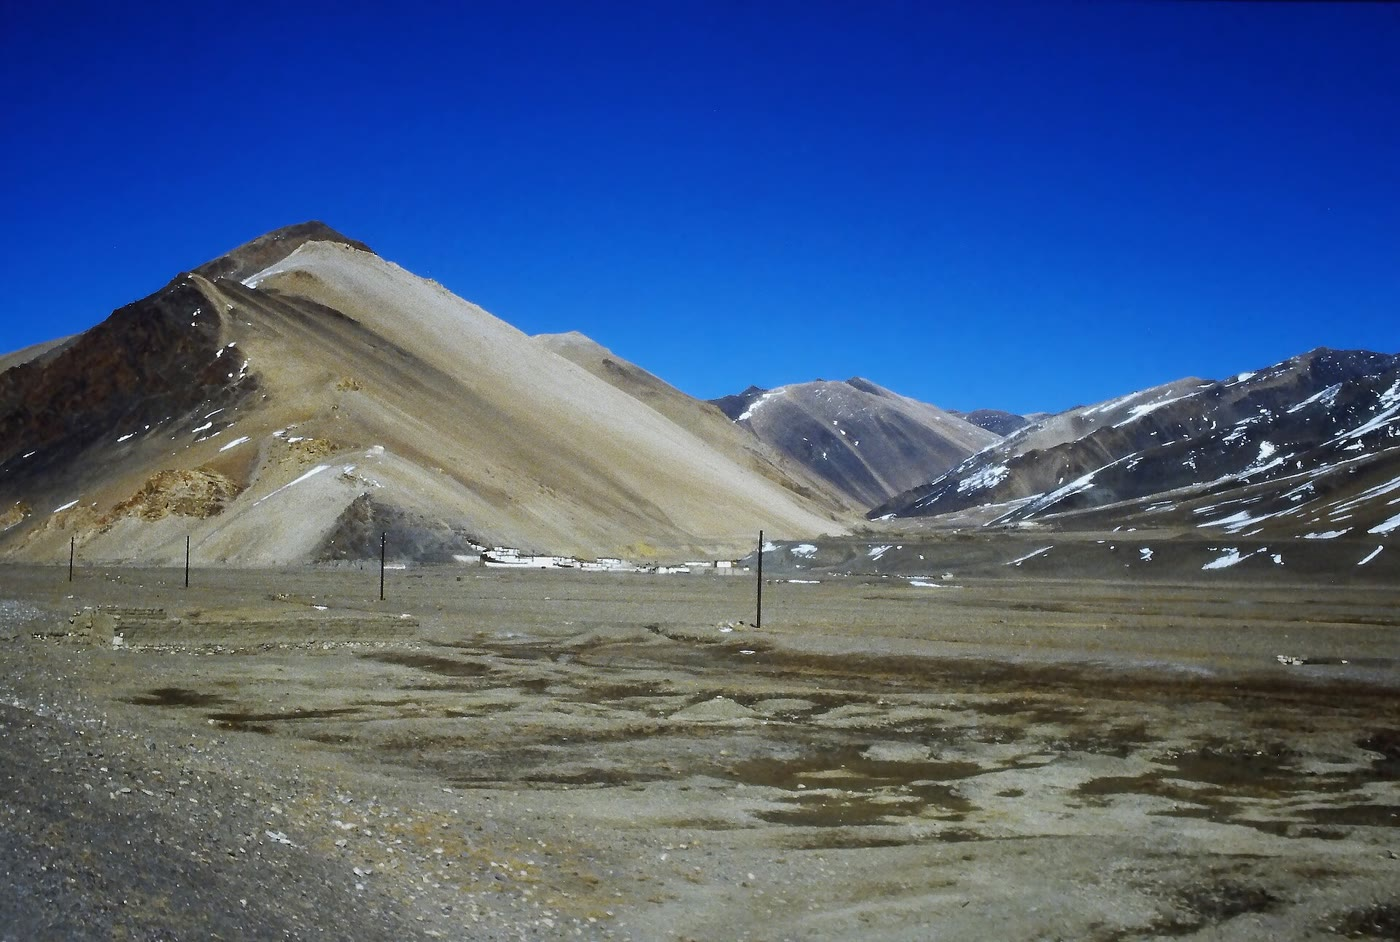
\includegraphics[width=0.66\linewidth]{images/book4/b2-14-tibet-plateau.jpg}
\par\smallskip{\small هضبة التبت بين نيبال وشيغاتسي: أرضية مستوية من الحصى
والمراعي المتناثرة، فيها قرية، بين جبال جرداء تكسوها الركامات السفحية، والكل على أكثر من
أربعة كيلومترات فوق مستوى سطح البحر.
الصورة: \mbox{\textdir TLT Jan Kranendonk, 1987, CC BY-SA 4.0}.}
\end{omfigure}
% ledger: data:b4-etopo-tibet

\subsection{ثقل الهضبة}

تثقل الهضبة على ما حولها. فعند كل عمق حتى قاعدة جذرها، يكون عمود
تحت الهضبة تحت ضغط أعلى من عمود تحت الأراضي المنخفضة المجاورة له؛
ولا يتساوى الاثنان إلا عند عمق التعويض. والعمود العالي يدفع نحو الخارج.

\begin{proposition}[فائض الطاقة الكامنة لهضبة]\label{prop:b2:himalaya-andes:gpe}
بفرضيات \cref{prop:b2:himalaya-andes:airy}، ومع الجاذبية $g$، يكون تكامل
فائض الضغط الصخري لعمود الهضبة على العمود العادي، من قمة
الهضبة إلى عمق التعويض عند قاعدة جذرها $r$، هو
\[
  \Delta F = \rho_c g h \left(H + \frac{h}{2} + \frac{r}{2}\right) .
\]
وهو فائض طاقة الوضع الثقالية لعمود الهضبة لكل وحدة مساحة،
والقوة لكل وحدة طول من حافة الهضبة التي تدفع بها الهضبة على
ما حولها.
\end{proposition}

\begin{proof}
قِس العمق $z$ نحو الأسفل من مستوى سطح البحر. في عمود الهضبة يكون الضغط $p_1 =
\rho_c g (z + h)$ من $z = -h$ إلى $L = H + r$. وفي العمود العادي يكون صفرًا فوق مستوى سطح
البحر، و$\rho_c g z$ في القشرة، و$\rho_c g H + \rho_m g (z - H)$ تحتها. والفرق $p_1
- p_0$ يرتفع من 0 عند $z = -h$ إلى $\rho_c g h$ عند مستوى سطح البحر؛ ويحتفظ بهذه القيمة عبر
القشرة العادية، حيث العمودان كلاهما قشرة؛ وتحت $z = H$ يتناقص خطيًا، بمقدار
$(\rho_m - \rho_c) g$ لكل متر، ويبلغ الصفر عند $L$ لأن $(\rho_m - \rho_c) r = \rho_c
h$. والتكامل هو مساحة شبه المنحرف هذا: $\rho_c g h\,(h/2 + H + r/2)$. والشغل الذي تبذله
الضغوط حين يتبادل العمودان المادة جانبيًا هو هذا التكامل، ولهذا فهو
يقيس الطاقة والدفع كليهما.
\end{proof}

\begin{omfigure}
\centering
% figdata/bachelor-2/plateaus.py part pressure (h = 4.8 km, H = 35 km, 2700 and 3300 kg/m3)
\begin{tikzpicture}
\begin{axis}[width=0.62\linewidth, height=5.6cm, y dir=reverse, xmin=0, xmax=160, ymin=-12,
  ymax=60, xlabel={فائض الضغط $p_1 - p_0$ \babelsublr{(\unit{MPa})}}, ylabel={العمق تحت مستوى سطح البحر
  \babelsublr{(\unit{km})}}, tick label style={font=\scriptsize}, label style={font=\small},
  xtick pos=bottom, ytick pos=left, clip=false]
\addplot[fill=omThm!20, draw=omThm, line width=1pt] table[x expr=\thisrow{p_high_MPa}-\thisrow{p_ref_MPa}, y=z_km] {figdata/out/bachelor-2-plateaus-pressure.dat} \closedcycle;
\draw[dashed] (axis cs:0,0) -- (axis cs:160,0);
\draw[dashed] (axis cs:0,35) -- (axis cs:160,35);
\draw[dashed] (axis cs:0,56.6) -- (axis cs:160,56.6);
\node[font=\scriptsize, anchor=north east] at (axis cs:160,0) {مستوى سطح البحر};
\node[font=\scriptsize, anchor=north east] at (axis cs:160,35) {\foreignlanguage{arabic}{الموهو العادي، $H$}};
\node[font=\scriptsize, anchor=south east] at (axis cs:160,56.6) {\foreignlanguage{arabic}{قاعدة الجذر، $H + r$}};
\node[font=\scriptsize, anchor=west] at (axis cs:100,-8.4) {\foreignlanguage{arabic}{قمة الهضبة، $-h$}};
\node[font=\scriptsize, align=center] at (axis cs:60,20) {\foreignlanguage{arabic}{المساحة $= \Delta F$}\\$\approx\qty{6.1e12}{N.m^{-1}}$};
\end{axis}
\end{tikzpicture}
\par\smallskip{\small فائض الضغط الصخري لعمود هضبة على عمود
عادي، من أجل $h = \qty{4.8}{km}$ و$H = \qty{35}{km}$ وكثافتين 2700
و\qty{3300}{kg.m^{-3}}: يرتفع عبر الهضبة، ويبقى عند $\rho_c g h = \qty{127}{MPa}$
عبر القشرة العادية، ويهبط إلى الصفر عند قاعدة الجذر. والمساحة المظلّلة هي
فائض الطاقة الكامنة في \cref{prop:b2:himalaya-andes:gpe}.}
\end{omfigure}
% values (plateaus.py): tibet_gpe 6.12179e12 N/m for h = 4.8

للتبت، $r = 4.5 \times 4.8 = \qty{21.6}{km}$ و$\Delta F = 2700 \times 9.8 \times 4800
\times (35000 + 2400 + 10800) \approx \qty{6.1e12}{N.m^{-1}}$. وإذا وُزّع على غلاف صخري
سمكه \qty{100}{km}، كان ذلك إجهادًا فائضًا متوسطًا قدره نحو \qty{60}{MPa}، من رتبة
الإجهادات التي تكسر الصخور. فهضبة بهذا الثقل لا يمكنها أن ترتفع ببساطة بعد ذلك: إنها تميل إلى الانبساط.

\begin{definition}[الانهيار الثقالي]\label{def:b2:himalaya-andes:collapse}
\emph{الانهيار الثقالي}\index{الانهيار الثقالي (لأوروجين)} لأوروجين
هو انبساط قشرته المتثخّنة تحت وزنها الذاتي، بتمدّد المناطق
العالية وبتدفّق نحو الخارج أو اندفاع عند الحواف، تحرّكه فائض الطاقة الكامنة
للأعمدة المتثخّنة.
\end{definition}

تتمدّد التبت بينما لا تزال الهند تدفعها. فعبر جنوب التبت، تقطع شقوق شمالية--جنوبية
الهضبة وتستوعب تمدّدًا شرقيًا--غربيًا: نحو $9 \pm \qty{2}{mm}$ في السنة
إجمالًا بين \ang{81} و\ang{92} شرقًا، و$1.3 \pm \qty{0.3}{mm}$ في السنة على شقّ يادونغ--غولو
وحده؛ وشمال نيبال تُظهر محطات GPS جنوب الهضبة يتمدّد بنحو
\num{12e-9} في السنة. والزلازل تروي القصة نفسها: فالتصدّع الدفعي \omterm{def:b2:himalaya-andes:thickening}{وتثخّن القشرة}
يسودان الأراضي المنخفضة المحيطة بالهضبة، والتصدّع المضربي والعادي داخلها.
أمّا لماذا تتمدّد فموضع خلاف. ففي الهضبة الشرقية قُرئ التمدّد على أنه انهيار
ثقالي يحرّكه وزن الهضبة؛ وفي الجنوب، يربطه آخرون بالشكل المقوّس
لقوس الهيمالايا، الذي تتباعد على امتداده الصدوع الدفعية، أو بانزلاق الهند تحتها.
% ledger: wang21:rifts, ader12:extension

\subsection{الإفلات جانبيًا}

\begin{definition}[البثق الجانبي]\label{def:b2:himalaya-andes:extrusion}
\emph{البثق الجانبي}\index{البثق الجانبي} (تكتونية الإفلات) هو طرد
كتل من القشرة أو الغلاف الصخري جانبيًا من نطاق تصادم، على امتداد صدوع مضربية كبيرة،
عموديًا تقريبًا على اتجاه التقارب، نحو حدّ حرّ.
\end{definition}

شرق التبت، لا تتقصّر آسيا فحسب؛ بل تُزاح جانبًا. فالصدوع المضربية اليسارية الطويلة،
ومنها صدعا النهر الأحمر وألتين تاغ، تُقرأ على أنها وجّهت
إفلات كتل كبيرة نحو الشرق والجنوب الشرقي، أولًا كتلة سوندا في جنوب شرق آسيا،
ثم التبت والصين الجنوبية، بينما انفتحت شقوق وأحواض محيطية فتيّة عند أطرافها البعيدة.
وقد أنتجت تجارب دُفع فيها قالب صلب في طبقة من الصلصال الاصطناعي صدوعًا كهذه؛ أمّا
النماذج التي عاملت آسيا صفيحةً لزجة متصلة فأنتجت بدلًا من ذلك تثخّنًا واسعًا، دون
صدوع كبرى. ويدعم نظام GPS حركة الكتل: فبالنسبة إلى سيبيريا المستقرة، يتحرك حوض
تاريم شمالًا تقريبًا بنحو \qty{14}{mm} في السنة، والصين الجنوبية نحو الشرق--الجنوب الشرقي
بنحو \qty{8}{mm} في السنة. أمّا كم من تقدّم الهند امتصّه التثخّن وكم
امتصّه البثق فلا يزال موضع جدل.
% ledger: jiao23:extrusion

\section{الأنديز}\label{sec:b2:himalaya-andes:andes}

تنزل صفيحة نازكا تحت أمريكا الجنوبية بنحو \qty{72}{mm} في السنة قرب خط العرض
\ang{20} جنوبًا، نحو الشرق--الشمال الشرقي، بحسب السرعات الزاوية لنموذج NNR-MORVEL56. لم تصل
أي قارة، ومع ذلك تحمل الأنديز الوسطى ثاني أعلى هضبة على الأرض.
% ledger: nnr56:poles
% values (plateaus.py): v_nazca_southamerica 72.52 mm/yr, azimuth 74.5

من الغرب إلى الشرق، بين نحو \ang{15} و\ang{27} جنوبًا، تضمّ خمسة نطاقات:
\emph{المنطقة الأمامية للقوس}؛ و\emph{الكورديليرا الغربية}، أي القوس البركاني؛ والهضبة العالية،
\emph{الألتيبلانو} في الشمال و\emph{البونا} في الجنوب؛ و\emph{الكورديليرا
الشرقية}؛ \omterm{def:b2:alpine-orogen:ftb}{وحزام الطيّات والدفع} الرقيق الجلد في \emph{النطاق تحت الأنديزي}، الذي
يتّصل بسهل تشاكو. ويعبرها المقطع أعلاه عند \ang{20} جنوبًا: فمن الخندق،
الذي تقع أعمق عقده على \qty{7.7}{km} تحت مستوى سطح البحر عند \ang{71.4} غربًا، يصعد السطح
أكثر من \qty{11}{km} في نحو \qty{240}{km} حتى حافة الهضبة عند \ang{69.1} غربًا؛
وتبقى الهضبة فوق \qty{3000}{m} على مدى \qty{440}{km} بمتوسط
قدره \qty{3760}{m}. ويبلغ متوسط الارتفاع \qty{3.7}{km} في الألتيبلانو و\qty{4.4}{km} في
البونا. وشمال \ang{23} جنوبًا يكون الموهو عمومًا أعمق من \qty{60}{km}؛ وتحت
الألتيبلانو الوسطى يبلغ سمك القشرة من 59 إلى \qty{64}{km}.
% ledger: gerbault05:andes, gerbault05:moho, data:b4-etopo-andes

\begin{omfigure}
\centering
\begin{tikzpicture}[x=0.56cm, y=0.38cm, font=\scriptsize]
% mantle background
\fill[gray!12] (0,-2.6) -- (5,-3.6) -- (8,-5.6) -- (10,-9.1) -- (12,-12.6) -- (13.2,-14.6) -- (26,-14.6)
  -- (26,-4.5) -- (20,-4.7) -- (17.5,-6.0) -- (15,-7.3) -- (11,-7.0) -- (9.5,-6.2) -- (8,-4) -- (5,-2)
  -- (0,-1) -- cycle;
% ocean water
\fill[blue!8] (0,0) -- (6.33,0) -- (5,-2) -- (0,-1) -- cycle;
% Nazca slab
\fill[gray!45] (0,-1) -- (5,-2) -- (8,-4) -- (10,-7.5) -- (12,-11) -- (14,-14.5) -- (13.2,-14.6)
  -- (12,-12.6) -- (10,-9.1) -- (8,-5.6) -- (5,-3.6) -- (0,-2.6) -- cycle;
% South American crust
\fill[orange!22] (5,-2) -- (8,1) -- (9,1.9) -- (10.2,2.0) -- (11,2.0) -- (15,2.0) -- (15.6,2.6) -- (16.8,2.4)
  -- (17.5,1.6) -- (20,0.6) -- (20.6,0.4) -- (26,0.3) -- (26,-4.5) -- (20,-4.7) -- (17.5,-6.0) -- (15,-7.3)
  -- (11,-7.0) -- (9.5,-6.2) -- (8,-4) -- cycle;
% Altiplano basin fill
\fill[yellow!45] (11,2.0) -- (15,2.0) -- (14.6,1.0) -- (11.4,1.0) -- cycle;
% surface line
\draw[line width=0.5pt] (0,-1) -- (5,-2) -- (8,1) -- (9,1.9) -- (10.2,2.0) -- (11,2.0) -- (15,2.0) -- (15.6,2.6)
  -- (16.8,2.4) -- (17.5,1.6) -- (20,0.6) -- (20.6,0.4) -- (26,0.3);
% arc volcanoes
\fill[red!60!black] (8.8,1.75) -- (9.2,2.9) -- (9.6,1.95) -- cycle;
\fill[red!60!black] (9.8,1.95) -- (10.2,2.8) -- (10.6,2.0) -- cycle;
\draw[red!60!black, decorate, decoration={snake, amplitude=0.6pt, segment length=4pt}] (10.8,-8.0) -- (9.9,1.6);
% Subandean decollement and splays
\draw[thick] (16.0,-1.2) -- (20.55,0.42);
\draw (17.4,-0.7) -- (17.85,1.45);
\draw (18.4,-0.35) -- (18.8,1.08);
\draw (19.4,0.0) -- (19.7,0.72);
% Moho
\draw[dashed] (8,-4) -- (9.5,-6.2) -- (11,-7.0) -- (15,-7.3) -- (17.5,-6.0) -- (20,-4.7) -- (26,-4.5);
% labels
\node at (2.6,-0.5) {الهادئ};
\node at (2.4,-2.2) {صفيحة نازكا};
\draw[-{Latex[length=1.6mm]}] (1.6,-2.8) -- (3.2,-3.0);
\node[anchor=south] (tr) at (4.3,0.9) {الخندق};
\draw[->] (tr.south) -- (5,-1.8);
\node[anchor=south east] at (7.6,1.0) {\shortstack{مقدّمة\\القوس}};
\node[anchor=south, align=center] at (9.7,3.0) {الكورديليرا\\\foreignlanguage{arabic}{الغربية (القوس)}};
\node[anchor=south] at (13,2.1) {الألتيبلانو};
\node[anchor=south, align=center] at (16.4,2.7) {الكورديليرا\\الشرقية};
\node[anchor=south west] at (18.6,1.3) {تحت الأنديزي};
\node[anchor=south] at (23.5,0.4) {سهل تشاكو};
\node at (13,-3.2) {قشرة سميكة};
\node at (23.2,-2.0) {الدرع البرازيلي};
\node[anchor=north] at (23.2,-4.6) {الموهو};
\node at (14.2,-9.6) {الإسفين الوشاحي};
\node at (21,-10) {الوشاح};
\node[rotate=-50] at (12.75,-12.9) {{\tiny الكتلة المندسّة}};
\draw[-{Latex[length=2mm]}] (1.2,4.6) -- (0.2,4.6);
\node[anchor=south] at (0.7,4.6) {\omnameCompassW};
\draw[-{Latex[length=2mm]}] (24.8,4.6) -- (25.8,4.6);
\node[anchor=south] at (25.3,4.6) {\omnameCompassE};
\end{tikzpicture}
\par\smallskip{\small مقطع تخطيطي عبر الأنديز الوسطى قرب \ang{20} جنوبًا (دون مقياس
رسم). تغوص صفيحة نازكا تحت المنطقة الأمامية للقوس؛ وتصعد \omterm{def:b2:magma-emplacement:magma}{الصهارة} من الإسفين الوشاحي (الخط
المتموّج) إلى قوس الكورديليرا الغربية؛ وتقع الألتيبلانو، بملئها الحوضي السميك،
بين الكورديليرتين، فوق قشرة سمكها نحو \qty{60}{km}؛ والحزام تحت الأنديزي الرقيق الجلد
مدفوع نحو الشرق فوق الدرع البرازيلي.}
\end{omfigure}
% ledger: gerbault05:andes, gerbault05:moho

\subsection{كيف صارت القشرة سميكة}

من أين جاءت القشرة الإضافية للألتيبلانو؟ المرشّح الأول هو التقصّر:
اضغط شريطًا من القشرة فيتثخّن، محتفظًا بمساحة مقطعه العرضي.

\begin{proposition}[التثخّن بالتقصّر]\label{prop:b2:himalaya-andes:shortening}
لتكن قشرة ذات سمك منتظم $H$ تقصّرت، دون كسب صخر أو فقده، إلى قشرة
سمكها $T$ على عرض $W$، والمقطع موازٍ للتقصّر. عندئذ كان
عرضها الأصلي $W_0 = W T/H$، والتقصّر هو
\[
  S = W_0 - W = W\,\frac{T - H}{H} .
\]
\end{proposition}

\begin{proof}
تُحفظ مساحة المقطع العرضي للقشرة، كما في توازن المساحة في
\cref{prop:b2:alpine-orogen:balance}: $W_0 H = W T$. ومنه $W_0 = WT/H$ و$S = W_0 - W =
W(T - H)/H$.
\end{proof}

عند \ang{20} جنوبًا يبلغ عرض الهضبة نحو \qty{440}{km}؛ فإن كانت قشرتها، التي يبلغ سمكها نحو \qty{60}{km}،
سمكها يومًا \qty{35}{km}، فالتقصّر اللازم هو $440 \times 25/35 \approx \qty{314}{km}$.
وتجد المقاطع المتوازنة قرب 16--\ang{21} جنوبًا نحو \qty{50}{km} من التقصّر في الألتيبلانو
وأكثر من \qty{200}{km} في النطاق تحت الأنديزي منذ الأوليغوسين. والأحجام القشرية
المحسوبة من التقصّر تقلّ بنحو \qty{20}{\percent} عن تلك المحسوبة من عمق
الموهو. وقد يعود جزء من الفرق إلى افتراضات خاطئة، عن السمك الأولي أو
عن طبيعة الموهو الزلزالي؛ وقد يكون جزء منه قشرة أُضيفت بطرق أخرى. وتنسب إحدى المجموعات قرب
\ang{21} جنوبًا إلى التقصّر التكتوني ما لا يقل عن \qty{55}{\percent} من الجذر، وإلى
تميّه وشاح الإسفين في المنطقة الأمامية للقوس ما يصل إلى \qty{20}{\percent}، وإلى الإضافة الصهارية
والتآكل التكتوني نحو \qty{5}{\percent} فقط. وقد يتحرّك الصخر أيضًا داخل الحزام:
فاختلافات سمك القشرة تخلق اختلافات في الطاقة الكامنة، كما في التبت،
وهذه يمكن أن تدفع القشرة السفلى الحارّة إلى التدفّق من السميك إلى الرقيق.
% ledger: gerbault05:andes, gerbault05:volume, gerbault05:moho, data:b4-etopo-andes

\begin{omfigure}
\centering
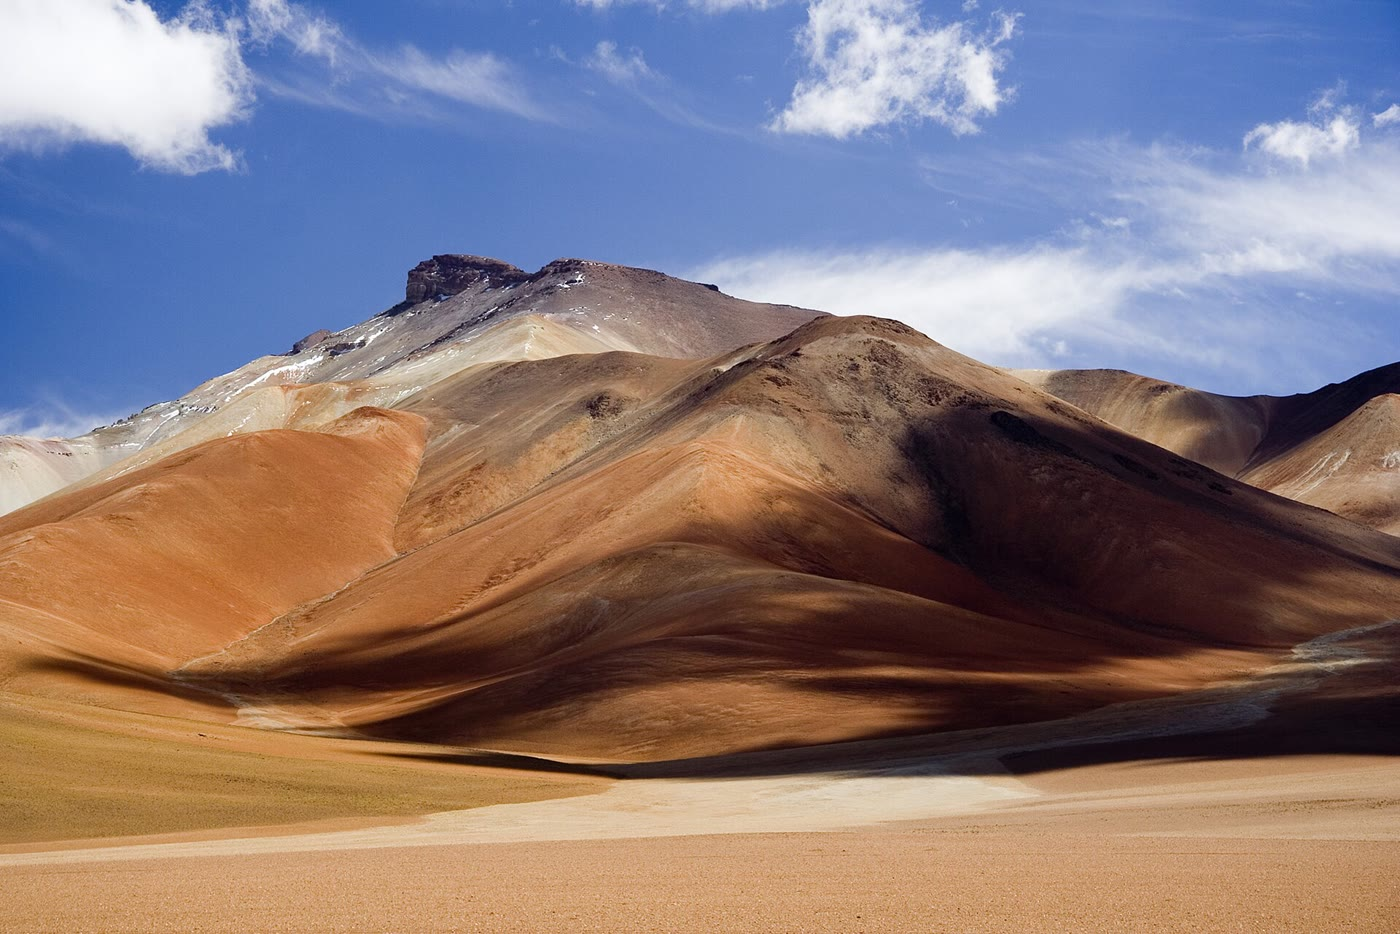
\includegraphics[width=0.66\linewidth]{images/book4/b2-14-altiplano.jpg}
\par\smallskip{\small الألتيبلانو البوليفية: سهل من الرمل والحصى عند سفوح
تلال جرداء تلوّنها صخورها بالأحمر والمغرة والرمادي. الصورة: \mbox{\textdir TLT Luca Galuzzi, 2006, CC BY-SA 2.5}.}
\end{omfigure}
% ledger: gerbault05:andes

\subsection{الكتل المسطّحة والجذور المفقودة}

زاوية الكتلة المندسّة ليست ثابتة، ولها أثرها على السطح.

\begin{definition}[الاندساس ذو الكتلة المسطّحة]\label{def:b2:himalaya-andes:flat-slab}
\emph{الاندساس ذو الكتلة المسطّحة}\index{الاندساس ذو الكتلة المسطّحة} اندساس تمتدّ فيه الكتلة المندسّة،
بعد نزولها الأول، أفقية تقريبًا تحت الصفيحة العليا مئات
الكيلومترات قبل أن تغوص من جديد.
\end{definition}

على امتداد الأنديز، قطعتان من كتلة نازكا المندسّة مسطّحتان اليوم: القطعة البيروفية، المسطّحة
منذ نحو \qty{15}{Ma}، والقطعة البامبية، منذ نحو \qty{18}{Ma}. وفوقهما لا توجد
براكين نشطة. فحين تسطّحت الكتلة البامبية، انتقل القوس نحو الداخل وقذف
حممًا أقل؛ وفوق القطعتين المسطّحتين سكت. وفجوة القوس والخندق في مجلد السنة الأولى
تفسّر الانتقال نحو الداخل: كلما قلّ ميل الكتلة تحت القوس، ابتعد عن الخندق الموضع الذي
تبلغ فيه العمق الذي ينصهر عنده الإسفين؛ والكتلة التي تبقى مسطّحة فوق ذلك العمق لا تترك
إسفينًا وشاحيًا حارًّا لينصهر على الإطلاق.
% ledger: gauthier24:flat

\begin{definition}[التقشّر الليثوسفيري]\label{def:b2:himalaya-andes:delamination}
\emph{التقشّر الليثوسفيري}\index{التقشّر الليثوسفيري} هو انفصال الجزء السفلي من غلاف صخري متثخّن،
أي غلافه الصخري الوشاحي وأحيانًا قشرة سفلى كثيفة، وغوصه في الأستينوسفير،
ليحلّ محلّه أستينوسفير حارّ.
\end{definition}

اقتُرح التقشّر تحت جنوب البونا، بين \ang{24} و\ang{27} جنوبًا، قبل
نحو 2 إلى \qty{3}{Ma}، حيث اندفعت حمم مافية فتيّة؛ وعلى امتداد الهضبة، رُبطت تغيّرات
سمك القشرة والارتفاع بغلاف صخري وشاحي أُزيل فعلًا
تحت جنوب الألتيبلانو ولم يُزل بعد كليًا تحت وسطها. وفقدان
غطاء وشاحي كثيف يجعل العمود الباقي أخفّ: فيرتفع السطح دون أي
تقصّر إضافي. وتقف البونا أعلى من الألتيبلانو بنحو \qty{1}{km} فوق قشرة أرقّ بنحو
\qty{11}{km}، وهو تباين يتطلّب إمّا قشرة أخفّ للبونا وإمّا وشاحًا أخفّ
تحتها.
% ledger: gerbault05:delamination, gerbault05:moho

\section{مقارنة بين الحزامين}\label{sec:b2:himalaya-andes:compared}

تبدو الهضبتان متشابهتين من بعيد وتختلفان في كل شيء آخر تقريبًا، كما يجمع الجدول
أدناه.

\begin{omfigure}
\centering\small
\begin{tabular}{>{\raggedright\arraybackslash}p{0.2\linewidth}|>{\raggedright\arraybackslash}p{0.34\linewidth}|>{\raggedright\arraybackslash}p{0.34\linewidth}}
 & الهيمالايا والتبت & الأنديز الوسطى \\ \hline
المحرّك & قارة في مواجهة قارة بعد انغلاق المحيط & صفيحة محيطية تغوص تحت قارة \\
المحور & درز تحفّه الأوفيوليتات & قوس بركاني فوق الكتلة المندسّة \\
الصهارية & مصهورات قشرية: ليوكوغرانيتات & أنديزيتات القوس؛ وحمم مافية حيث فُقد الغلاف الصخري \\
التقارب & نحو \qty{45}{mm} في السنة، تأخذ السلسلة نصفه & نحو \qty{72}{mm} في السنة، يستهلك الاندساس معظمه \\
الزلازل الكبرى & على MHT، آسام 1950، $M_w \approx 8.5$ & على سطح الاندساس، تشيلي 1960، قدر عزمه $M_w$ يبلغ 9.5 \\
الهضبة & متوسط \qty{4.8}{km} على \qty{1180}{km}؛ قشرة من 70 إلى \qty{75}{km} & متوسط \qty{3.8}{km} على \qty{440}{km}؛ قشرة نحو \qty{60}{km} \\
تكتونية الهضبة & تمدّد شرقي--غربي، بثق & تقصّر على الجانبين؛ تقشّر مقترح \\
المقدّمة & المنخفض الأمامي الهندي--الغانجي ومولاس سيواليك & الحزام تحت الأنديزي وسهل تشاكو \\
\end{tabular}
\par\smallskip{\small الحزامان جنبًا إلى جنب؛ المصادر مذكورة في الأقسام أعلاه،
وزلزال تشيلي هو الأكبر المسجّل منذ عام 1900.}
\end{omfigure}
% ledger: lave00:setting, lave00:siwaliks, weinberg16:himalaya, ader12:mht, ader12:quakes, usgs:largest, gerbault05:andes, gerbault05:moho, gerbault05:delamination, nnr56:poles, data:b4-etopo-tibet, data:b4-etopo-andes, cattin01:crust, wang21:rifts, jiao23:extrusion

أعمق الفروق فيما ينزل. ففي الأنديز تستمر الصفيحة المحيطية في الغوص،
ويُستهلك معظم التقارب، نحو \qty{72}{mm} في السنة، عند الخندق؛ وتقصير
الصفيحة العليا بمقدار \qty{310}{km} على مدى نحو 30 مليون سنة لا يأخذ منه إلا نحو \qty{10}{mm} في
السنة. وفي الهيمالايا لا شيء خفيفًا يمكنه أن يغوص طويلًا، فيُنفق التقارب في
التكديس والتثخين ودفع آسيا جانبًا. ويُنمّي كلا الحزامين هضبة لأن القشرة السميكة
قشرة عالية؛ وتتوقف كلتا الهضبتين عن الارتفاع حين يوازن وزنها الذاتي الدفع عند
حوافها، ثم تنبسطان.
% ledger: nnr56:poles, gerbault05:andes, ader12:mht, jiao23:extrusion

\section{إلى أي ارتفاع يمكن أن يبلغ جبل؟}\label{sec:b2:himalaya-andes:heights}

تقف أعلى قمة، إفرست، على ارتفاع \qty{8848.86}{m} فوق مستوى سطح البحر بحسب المسح المشترك
المعلن عام 2020. فلماذا ليس عشرين كيلومترًا؟ يأتي حدّ تقريبي من مقاومة الصخر.

\begin{proposition}[حدّ للارتفاع من مقاومة الصخر]\label{prop:b2:himalaya-andes:height}
عمود من الصخر كثافته $\rho$ يقف على ارتفاع $h$ فوق ما حوله، دون
إسناد جانبي فوق مستواها، يحمل عند قدمه إجهادًا رأسيًا $\rho g h$
وإجهادًا أفقيًا صفريًا على جوانبه الحرّة، ومن ثمّ إجهادًا تفاضليًا $\rho g h$. فإذا كان
الصخر ينكسر عند الإجهاد التفاضلي $\sigma_d$، فإن العمود لا يقف إلا إذا كان $h < \sigma_d/(\rho
g)$.
\end{proposition}

\begin{proof}
عند قدم العمود يكون الإجهاد الرأسي وزن الصخر الذي فوقه لكل وحدة مساحة،
$\rho g h$. والجوانب حرّة، فالإجهاد الأفقي هناك صفر. والإجهاد التفاضلي
هو الفرق بين أكبر الإجهادات الرئيسية وأصغرها، وهو هنا $\rho g h - 0$.
ولا يُتجنّب الانكسار إلا إذا بقي دون $\sigma_d$.
\end{proof}

للجبل الحقيقي جوانب منحدرة تمسك لبّه، فيكون الإجهاد تحته
أصغر؛ وكرتبة مقدار خذ النصف، $\rho g h/2$. ولإفرست، $2700 \times 9.8
\times 8849/2 \approx \qty{117}{MPa}$. ويضع قانون بايرلي في مجلد السنة الأولى المقاومة
الاحتكاكية للصخر على صدع تحت إجهاد عمودي قدره \qty{200}{MPa} عند $50 + 0.6 \times 200 =
\qty{170}{MPa}$: الرتبة نفسها. فالجبل الأعلى بثلاث مرات سيُحمّل قاعدته بما يتجاوز كثيرًا
ما يحتمله الصخر؛ فينكسر وينبسط. وعلى الأرض، القمم التي يبلغ ارتفاعها ثمانية إلى تسعة كيلومترات
قريبة من الحدّ، والهضبة، التي تنبسط قبل أن تنكسر قممها بزمن طويل، تستقر
عند خمسة.
% ledger: tht:everest, byerlee:1975

\section*{التمارين}\label{sec:b2:himalaya-andes:exercises}

معطيات التمارين: $g = \qty{9.8}{m.s^{-2}}$؛ وكثافتا القشرة والوشاح
\qty{2700}{kg.m^{-3}} و\qty{3300}{kg.m^{-3}} ما لم يُذكر غير ذلك؛ والقشرة العادية $H =
\qty{35}{km}$.

\begin{exercise}[$\star$]\label{exo:b2:himalaya-andes:1}
تقف هضبة على متوسط ارتفاع قدره \qty{3.0}{km}. باستعمال
\cref{prop:b2:himalaya-andes:airy}، احسب (أ) جذرها وفق إيري، (ب) سمك قشرتها.
(ج) بكم ترفعها \qty{10}{km} إضافية من القشرة؟
\end{exercise}

\begin{exercise}[$\star$]\label{exo:b2:himalaya-andes:2}
يمتدّ مقطع عبر هيمالايا نيبال من سهل الغانج إلى هضبة التبت.
(أ) عدّد، بالترتيب، الوحدات التي يعبرها والصدوع التي تفصل بينها. (ب) أي صدع
هو صدع عادي؟ (ج) كيف تتغيّر الدرجة التحوّلية نحو الشمال حتى متتالية الهيمالايا
الكبرى، ثم فوقها؟
\end{exercise}

\begin{exercise}[$\star$]\label{exo:b2:himalaya-andes:3}
في وسط نيبال تعرّضت مصطبة نهرية هُجرت قبل \qty{9.2}{kyr} لتقصّر قدره
\qty{196.5}{m} عبر طيّات الصدع الدفعي الجبهي الرئيسي. (أ) احسب معدّل التقصّر
المتوسط بالمليمترات في السنة. (ب) قارنه بتقارب GPS عبر السلسلة،
\qty{17.8}{mm} في السنة. (ج) ماذا يقول هذا التوافق عن الصدوع الواقعة شمال MFT؟
\end{exercise}

\begin{exercise}[$\star$]\label{exo:b2:himalaya-andes:4}
صنّف كل ملاحظة في خانة \omterm{def:b2:himalaya-andes:types}{الأوروجين التصادمي} أو \omterm{def:b2:himalaya-andes:types}{الأوروجين من النمط الأنديزي} أو كليهما: (أ) درز تحفّه
الأوفيوليتات؛ (ب) خط من البراكين الأنديزيتية النشطة؛ (ج) ليوكوغرانيتات منصهرة من
القشرة؛ (د) خندق محيطي عميق على امتداد الجبهة؛ (ه) حوض أمامي جبلي فيه مولاس؛
(و) زلازل كبرى على صدع قليل الميل تحت السلسلة.
\end{exercise}

\begin{exercise}[$\star\star$]\label{exo:b2:himalaya-andes:5}
تتحرك الهند بسرعة \qty{45}{mm} في السنة بالنسبة إلى أوراسيا عبر الهيمالايا؛ وعبر نيبال
تمتصّ السلسلة نفسها \qty{17.8}{mm} في السنة في الشرق و\qty{20.5}{mm} في السنة في الغرب.
(أ) ما نسبة التقارب التي تأخذها السلسلة في كل حالة؟ (ب) أين يذهب
الباقي؟ (ج) على مدى \qty{10}{Myr}، كم من التقصّر يمثّل الباقي؟
\end{exercise}

\begin{exercise}[$\star\star$]\label{exo:b2:himalaya-andes:6}
(أ) باستعمال \cref{prop:b2:himalaya-andes:gpe}، احسب فائض الطاقة الكامنة
للألتيبلانو، التي يبلغ متوسط ارتفاعها \qty{3.7}{km}. (ب) قارنه بفائض التبت عند \qty{4.8}{km}.
(ج) بيّن أنه لهضبة رقيقة، $h \ll H$، ينمو $\Delta F$ متناسبًا مع $h$، وأنه لهضبة
سميكة ينمو أسرع: ماذا يعني ذلك لنموّ الهضبة؟
\end{exercise}

\begin{exercise}[$\star\star$]\label{exo:b2:himalaya-andes:7}
(أ) احسب $\rho g h/2$ تحت إفرست، التي يبلغ ارتفاعها \qty{8848.86}{m}، مع $\rho =
\qty{2700}{kg.m^{-3}}$. (ب) بحسب قانون بايرلي، $\tau = 0.85\,\sigma_n$ دون \qty{200}{MPa} من
الإجهاد العمودي و$\tau = \qty{50}{MPa} + 0.6\,\sigma_n$ فوقها؛ احسب $\tau$ من أجل $\sigma_n =
100$ و\qty{200}{MPa}. (ج) ما الارتفاع الذي تسمح به مقاومة قدرها \qty{170}{MPa}، بقاعدة
رتبة المقدار نفسها؟
\end{exercise}

\begin{exercise}[$\star\star$]\label{exo:b2:himalaya-andes:8}
تستوعب الشقوق في جنوب التبت $9 \pm \qty{2}{mm}$ في السنة من التمدّد الشرقي--الغربي بين
\ang{81} و\ang{92} شرقًا. (أ) ما عرض هذا المدى عند \ang{30} شمالًا، مع \qty{111.19}{km} لكل
درجة على خط الطول؟ (ب) احسب معدّل الانفعال التمدّدي المتوسط، في السنة وفي الثانية،
مع مداه. (ج) قارن بالقيمة $(12.4 \pm 4.7) \times 10^{-9}$ في السنة المستخرجة من GPS شمال نيبال.
\end{exercise}

\begin{exercise}[$\star\star$]\label{exo:b2:himalaya-andes:9}
يراكم الصدع الدفعي الهيمالايي الرئيسي المقفل تحت نيبال عجزًا في العزم قدره
\qty{6.6e19}{N.m} في السنة؛ ولم تحرّر زلازل آخر 500 سنة إلا
\qty{0.9e19}{N.m} في السنة. (أ) ما نسبة العجز التي حرّرتها؟ (ب) مع $M_0 =
10^{1.5 M_w + 9.1}$\,\unit{N.m}، احسب عزم زلزال قدر عزمه $M_w$ يبلغ 8.5. (ج) كم مرة
يلزم وقوع زلازل كهذه لموازنة العجز؟
\end{exercise}

\begin{exercise}[$\star\star\star$]\label{exo:b2:himalaya-andes:10}
تقف البونا أعلى من الألتيبلانو بمقدار \qty{0.7}{km} (4.4 مقابل \qty{3.7}{km}) فوق قشرة
أرقّ بمقدار \qty{11}{km}. خذ قشرة الألتيبلانو بسمك \qty{61.5}{km} وكثافة
\qty{2800}{kg.m^{-3}}، ووشاحًا كثافته \qty{3300}{kg.m^{-3}} تحت كلتيهما. (أ) اكتب
تساوي كتلتي العمودين فوق عمق تعويض مشترك. (ب) أوجد
الكثافة التي يجب أن تكون لقشرة البونا إذا عوّضت القشرة وحدها الفرق. (ج) قارن
بالقيم من 150 إلى \qty{200}{kg.m^{-3}} المذكورة، وقل ما الذي يمكن أن يفسّر التباين أيضًا.
\end{exercise}

\begin{exercise}[$\star\star\star$]\label{exo:b2:himalaya-andes:11}
تقف الجبهة البركانية حيث يكون سطح الكتلة المندسّة على عمق \qty{105}{km}. (أ) لكتلة
مائلة ميلًا منتظمًا بالزاوية \ang{30}، احسب فجوة القوس والخندق بصيغة مجلد السنة
الأولى. (ب) صارت الكتلة الآن تميل بالزاوية \ang{30} حتى \qty{90}{km}، ثم بالزاوية \ang{4} فقط: احسب
الفجوة الجديدة وانتقال القوس نحو الداخل. (ج) ماذا يحدث للقوس إذا تسطّحت الكتلة
على عمق \qty{95}{km} وبقيت هناك على مدى \qty{300}{km}؟
\end{exercise}

\begin{exercise}[$\star\star\star$]\label{exo:b2:himalaya-andes:12}
يزيل الحتّ نحو \qty{300}{km^3} من الصخر لكل كيلومتر من الهيمالايا في كل مليون سنة.
وتأتي الهند بقشرة سمكها \qty{37.5}{km} بسرعة \qty{21}{mm} في السنة. (أ) كم من القشرة لكل
كيلومتر من السلسلة في كل مليون سنة يدخل الحزام؟ (ب) ما النسبة التي يزيلها الحتّ؟
(ج) أين يمكن أن يكون الباقي؟
\end{exercise}

\begin{problem}[{مسألة نهاية الأسبوع --- هضبتان}]\label{pb:b2:himalaya-andes:1}
تعطي مقاطع الشرائط في هذا الفصل متوسط ارتفاع العقد عبر التبت
(\qtyrange{86}{90}{\degree} شرقًا) وعبر الأنديز الوسطى (\qtyrange{19}{21}{\degree} جنوبًا).
وإذا أُخذت عيّناتها كل \ang{1.5} من خطوط العرض وكل درجة من خطوط الطول، مدوّرة إلى \qty{10}{m}، فإنها
تُقرأ كما يلي. وما لم يُذكر غير ذلك، $g = \qty{9.8}{m.s^{-2}}$ و$\rho_c = \qty{2700}{kg.m^{-3}}$
و$\rho_m = \qty{3300}{kg.m^{-3}}$ وسمك القشرة العادية $H = \qty{35}{km}$.

\smallskip
\begin{center}\small
\begin{tabular}{l|ccccccccc}
خط العرض (\unit{\degree} شمالًا) & 26.5 & 28.0 & 29.5 & 31.0 & 32.5 & 34.0 & 35.5 & 37.0 & 38.5 \\ \hline
متوسط الارتفاع (\unit{m}) & 70 & 5000 & 5030 & 4830 & 5020 & 5150 & 5050 & 4470 & 2210
\end{tabular}

\smallskip
\begin{tabular}{l|cccccccc}
خط الطول (\unit{\degree}) & $-71$ & $-70$ & $-69$ & $-68$ & $-67$ & $-66$ & $-65$ & $-64$ \\ \hline
متوسط الارتفاع (\unit{m}) & $-3310$ & 970 & 4150 & 3720 & 3740 & 4010 & 3030 & 1170
\end{tabular}
\end{center}
\smallskip

\noindent\textbf{الجزء الأول --- قراءة المقاطع.}
\begin{enumerate}
\item باعتبار الهضبة هي العيّنات التي تزيد على \qty{3000}{m}، احسب متوسط ارتفاع التبت
$h_T$، مدوّرًا إلى \qty{0.1}{km}.
\item افعل الشيء نفسه للألتيبلانو، $h_A$، وقارن بمتوسط الارتفاع
\qty{3.7}{km} المذكور للألتيبلانو و\qty{4.4}{km} للبونا.
\item ما عرض كل هضبة، على الأقل، بحسب العيّنات (\qty{111.19}{km} لكل
درجة عرض؛ و\qty{104.5}{km} لكل درجة طول عند \ang{20} جنوبًا)؟
\item احسب الميل المتوسط لجبهة الهيمالايا بين \ang{26.5} و\ang{28.0} شمالًا، في صورة
نسبة مئوية.
\item لماذا المقطع الأنديزي أشدّ لاتناظرًا بكثير من المقطع التبتي؟
\end{enumerate}

\noindent\textbf{الجزء الثاني --- سماكات إيري.}
\begin{enumerate}[resume]
\item احسب جذر إيري وسمك القشرة $T_T$ للتبت من $h_T$.
\item افعل الشيء نفسه للألتيبلانو، $T_A$.
\item قارن بالسماكات الزلزالية، من 70 إلى \qty{75}{km} تحت التبت ومن 59 إلى
\qty{64}{km} تحت وسط الألتيبلانو. أي التقديرين أبعد عن الواقع؟
\item ما كثافة القشرة التي تجعل سمك إيري للتبت مساويًا \qty{72.5}{km}؟
\item ما الكثافة التي تعطي \qty{61.5}{km} للألتيبلانو؟
\item اذكر سببين، غير كثافة القشرة، يجعلان حساب إيري المحلي
يخطئ الجذر المرصود.
\item يبلغ سمك القشرة \qty{37.5}{km} تحت الهند و\qty{72.5}{km} تحت التبت. مع
تباين كثافة عند الموهو قدره \qty{370}{kg.m^{-3}}، قدّر بصفيحة بوغيه، $\Delta g
= 2\pi G\,\Delta\rho\,t$، شذوذ بوغيه لجذر التبت بالنسبة إلى الهند، حيث $t$
السمك الإضافي تحت مستوى سطح البحر ($G = \qty{6.674e-11}{m^3.kg^{-1}.s^{-2}}$). وقارن بالفرق
المرصود البالغ \qty{460}{mGal}.
\end{enumerate}

\noindent\textbf{الجزء الثالث --- تقصير الألتيبلانو.} عند \ang{20} جنوبًا يبلغ عرض الهضبة
\qty{440}{km} وسمك قشرتها نحو \qty{60}{km}.
\begin{enumerate}[resume]
\item باستعمال \cref{prop:b2:himalaya-andes:shortening}، احسب العرض المُرجَع
والتقصّر اللازم إذا كان سمك القشرة \qty{35}{km} من قبل.
\item تعطي المقاطع المتوازنة نحو \qty{50}{km} من التقصّر في الألتيبلانو
و\qty{200}{km} في النطاق تحت الأنديزي. ما نسبة التقصّر اللازم المفقودة؟
\item إذا لم يصنع التقصّر إلا \qty{55}{\percent} من القشرة الإضافية، فكم من التقصّر
يلزم؟
\item الحزام تحت الأنديزي رقيق الجلد. لماذا يجب أن يُثخّن تقصّره القشرة مع ذلك
في مكان ما؟
\item افترض أن \qty{314}{km} في الجزء الثالث تراكمت على مدى \qty{30}{Myr}. احسب المعدّل
المتوسط، ونسبة ما يمثّله من تقارب نازكا--أمريكا الجنوبية الحالي، \qty{72}{mm} في السنة.
\item أين يذهب باقي التقارب؟
\end{enumerate}

\noindent\textbf{الجزء الرابع --- ثقل التبت.}
\begin{enumerate}[resume]
\item باستعمال \cref{prop:b2:himalaya-andes:gpe} مع $h_T$، احسب فائض الطاقة
الكامنة للتبت لكل وحدة مساحة.
\item احسبه للألتيبلانو مع $h_A$، والنسبة بين الاثنين.
\item وزّع $\Delta F$ للتبت على غلاف صخري سمكه \qty{100}{km}: ما الإجهاد المتوسط الذي
يمثّله؟
\item كم يبلغ الانفعال في السنة لتمدّد جنوب التبت، \qty{9}{mm} في السنة عبر \qty{1060}{km}؟
\item لماذا يمكن للتبت أن تتمدّد شرقًا--غربًا بينما لا تزال الهند تدفعها نحو الشمال؟
\item خلاصة: أعطِ سمك قشرة التبت المحسوب من متوسط ارتفاعها، مدوّرًا
إلى الكيلومتر، ونسبة ما يفسّره من السمك الزلزالي \qty{72.5}{km}.
\end{enumerate}
\end{problem}
